%% This is file `sigconf.tex',
%% generated with the docstrip utility.
%%
%% The original source files were:
%%
%% samples.dtx  (with options: `all,proceedings,sigconf')
%%
%% IMPORTANT NOTICE:
%%
%% For the copyright see the source file.
%%
%% Any modified versions of this file must be renamed
%% with new filenames distinct from sigconf.tex.
%%
%% For distribution of the original source see the terms
%% for copying and modification in the file samples.dtx.
%%
%% This generated file may be distributed as long as the
%% original source files, as listed above, are part of the
%% same distribution. (The sources need not necessarily be
%% in the same archive or directory.)
%%
%%
%% Commands for TeXCount
%TC:macro \cite [option:text,text]
%TC:macro \citep [option:text,text]
%TC:macro \citet [option:text,text]
%TC:envir table 0 1
%TC:envir table* 0 1
%TC:envir tabular [ignore] word
%TC:envir displaymath 0 word
%TC:envir math 0 word
%TC:envir comment 0 0
%%
%% The first command in your LaTeX source must be the \documentclass
%% command.
%%
%% For submission and review of your manuscript please change the
%% command to \documentclass[manuscript, screen, review]{acmart}.
%%
%% When submitting camera ready or to TAPS, please change the command
%% to \documentclass[sigconf]{acmart} or whichever template is required
%% for your publication.
%%
%%
\PassOptionsToPackage{draft}{microtype}
\documentclass[sigconf, language=english, language=brazilian,natbib=false]{acmart}
%%
%% \BibTeX command to typeset BibTeX logo in the docs
\AtBeginDocument{%
  \providecommand\BibTeX{{%
    Bib\TeX}}}

%% Rights management information.  This information is sent to you
%% when you complete the rights form.  These commands have SAMPLE
%% values in them; it is your responsibility as an author to replace
%% the commands and values with those provided to you when you
%% complete the rights form.
\setcopyright{none}                          % remove o bloco de direitos autorais
\settopmatter{printacmref=false}             % remove o "ACM Reference Format"
\renewcommand\footnotetextcopyrightpermission[1]{} % remove o rodapé de permissão
\settopmatter{printfolios=true}
\acmConference[Qualidade de Software 2026/2]{Qualidade de Software 2026/2}{}{}
% cabeçalho: evita as vírgulas sobrando (data e local vazios)
\makeatletter
\AtBeginDocument{%
  \fancyhead[LE]{\ACM@linecountL\@headfootfont\footnotesize Qualidade de Software 2026/2}%
  \fancyhead[RO]{\@headfootfont Qualidade de Software 2026/2\ACM@linecountR}%
}
\makeatother


%%
%% For managing citations, it is recommended to use bibliography
%% files in BibTeX format.
%%
%% You can then either use BibTeX with the ACM-Reference-Format style,
%% or BibLaTeX with the acmnumeric or acmauthoryear sytles, that include
%% support for advanced citation of software artefact from the
%% biblatex-software package, also separately available on CTAN.
%%
%% Look at the sample-*-biblatex.tex files for templates showcasing
%% the biblatex styles.
%%
%%
%% The majority of ACM publications use numbered citations and
%% references.  The command \citestyle{authoryear} switches to the
%% "author year" style.
%%
%% If you are preparing content for an event
%% sponsored by ACM SIGGRAPH, you must use the "author year" style of
%% citations and references.
%% Uncommenting
%% the next command will enable that style.
%%\citestyle{acmauthoryear}

\usepackage[
    backend=biber,
    style=acmnumeric,
    sorting=none
]{biblatex}
\usepackage{float}
\usepackage{placeins}
\addbibresource{sigconf.bib}
%%
%% end of the preamble, start of the body of the document source.
\begin{document}

%%
%% The "title" command has an optional parameter,
%% allowing the author to define a "short title" to be used in page headers.
\title[Avaliação da Qualidade de Produto - Khan Academy]{Avaliação da Qualidade de Produto de Software \\ \large Khan Academy}

\author{Camila Silva Cavalcante}
\email{camilacsc08@gmail.com}
\affiliation{%
  \institution{Matrícula 232013944}
  \country{Brazil}
}

\author{Enzo Menali Vettorato Toledo}
\email{enzomenali@gmail.com}
\affiliation{%
  \institution{Matrícula 241011054}
  \country{Brazil}
}

\author{Geovanna Alves Umbelino}
\email{geovannaalves.u@gmail.com}
\affiliation{%
  \institution{Matrícula 232014450}
  \country{Brazil}
}

\author{José Augusto Alves de Moraes}
\email{joseaugustomoraes@protonmail.com}
\affiliation{%
  \institution{Matrícula 231026429}
  \country{Brazil}
}

\author{Luísa de Souza Ferreira}
\email{luisasouzalinda90@gmail.com}
\affiliation{%
  \institution{Matrícula 232014807}
  \country{Brazil}
}

\author{Pedro Lucas Barbosa da Silva}
\email{21pedrolucas21@gmail.com}
\affiliation{%
  \institution{Matrícula 241025710}
  \country{Brazil}
}

\renewcommand{\shortauthors}{Irmã Mary Keller}

%%
%% The abstract is a short summary of the work to be presented in the
%% article.

\begin{abstract}
Este trabalho avalia a qualidade da plataforma web da Khan Academy segundo a família de normas ISO/IEC 25000 (SQuaRE), com foco em eficiência de desempenho, portabilidade e usabilidade, selecionadas por uma matriz ponderada com classificação MoSCoW. A especificação segue a abordagem \textit{Goal Question Metric} (GQM), com três objetivos, 11 questões e 14 métricas, a serem aplicadas por testes externos de caixa-preta em navegadores de computador.
\end{abstract}

\begin{translatedabstract}{english}
This paper evaluates the quality of Khan Academy's web platform according to the ISO/IEC 25000 (SQuaRE) series, focusing on performance efficiency, portability, and usability, selected through a weighted matrix with MoSCoW classification. The specification follows the \textit{Goal Question Metric} (GQM) approach, with three goals, 11 questions, and 14 metrics, to be applied through external black-box testing on desktop browsers.
\end{translatedabstract}

%%
%% The code below is generated by the tool at http://dl.acm.org/ccs.cfm.
%% Please copy and paste the code instead of the example below.
%%
\begin{CCSXML}
<ccs2012>
<concept>
<concept_id>10011007.10011074.10011099.10011693</concept_id>
<concept_desc>Software and its engineering~Empirical software validation</concept_desc>
<concept_significance>500</concept_significance>
</concept>
<concept>
<concept_id>10003120.10003121.10003122.10010854</concept_id>
<concept_desc>Human-centered computing~Usability testing</concept_desc>
<concept_significance>500</concept_significance>
</concept>
<concept>
<concept_id>10003120.10011738.10011774</concept_id>
<concept_desc>Human-centered computing~Accessibility design and evaluation methods</concept_desc>
<concept_significance>500</concept_significance>
</concept>
<concept>
<concept_id>10010405.10010489.10010495</concept_id>
<concept_desc>Applied computing~E-learning</concept_desc>
<concept_significance>500</concept_significance>
</concept>
</ccs2012>
\end{CCSXML}

\ccsdesc[500]{Software and its engineering~Empirical software validation}
\ccsdesc[500]{Human-centered computing~Usability testing}
\ccsdesc[500]{Human-centered computing~Accessibility design and evaluation methods}
\ccsdesc[500]{Applied computing~E-learning}

%%
%% Keywords. The author(s) should pick words that accurately describe
%% the work being presented. Separate the keywords with commas.

\keywords{SQuaRE, ISO/IEC 25010, GQM, Eficiência de Desempenho, Portabilidade, Usabilidade, Khan Academy}
%%
%% This command processes the author and affiliation and title
%% information and builds the first part of the formatted document.
\maketitle


\section{Introdução}
O uso de plataformas digitais na educação tem ampliado as possibilidades de acesso ao conhecimento e de acompanhamento da aprendizagem. Entretanto, a adoção dessas ferramentas exige atenção à qualidade do software, especialmente em aspectos como desempenho, acessibilidade e adaptação a diferentes ambientes computacionais. Essas características são particularmente relevantes em contextos educacionais com limitações de infraestrutura tecnológica.

A Khan Academy é uma plataforma educacional que oferece videoaulas, exercícios interativos e recursos de acompanhamento do progresso dos estudantes. Considerando a diversidade de usuários e condições de acesso, torna-se importante avaliar se a plataforma apresenta características de qualidade adequadas às necessidades de estudantes, professores e responsáveis.

Diante desse cenário, este trabalho tem como objetivo avaliar a qualidade da versão web da Khan Academy, com foco em três características da \textbf{ISO/IEC 25010:2011 \cite{iso25010}: eficiência de desempenho, portabilidade e usabilidade.} A avaliação contempla comportamento temporal, utilização de recursos, adaptabilidade, acessibilidade e apreensibilidade, considerando os fluxos de navegação em cursos, reprodução de videoaulas, resolução de exercícios e consulta ao progresso do estudante.

Para conduzir a avaliação, adota-se o processo de avaliação de produtos de software da família SQuaRE \cite{iso25000,iso25040}, utilizando a abordagem GQM para relacionar objetivos, questões e métricas, com referência à ISO/IEC 25023:2016 \cite{iso25023}. A investigação será realizada por meio de testes externos à plataforma web, com foco em comportamentos observáveis, buscando identificar limitações e oportunidades de melhoria fundamentadas nas evidências coletadas.


\section{Referencial Teórico}

\subsection{Qualidade de Software e Modelo SQuaRE}

A qualidade de software está relacionada à capacidade de um produto atender às necessidades e expectativas de seus usuários, considerando características que influenciam seu funcionamento e sua utilização. Para apoiar a avaliação dessas características, a família de normas ISO/IEC 25000, denominada \textit{Systems and Software Quality Requirements and Evaluation} (SQuaRE) \cite{iso25000}, estabelece modelos e diretrizes para a especificação e avaliação da qualidade de produtos de software.

Entre essas normas, a ISO/IEC 25010:2011 \cite{iso25010} apresenta um modelo de qualidade que permite organizar as características e subcaracterísticas a serem avaliadas. Complementarmente, a ISO/IEC 25023:2016 \cite{iso25023} estabelece medidas que auxiliam na obtenção de evidências quantitativas sobre a qualidade do produto, contribuindo para avaliações estruturadas e fundamentadas em critérios definidos.

\subsection{Características de Qualidade}

A ISO/IEC 25010:2011 \cite{iso25010} organiza a qualidade de produto em oito características, das quais três foram priorizadas neste estudo: eficiência de desempenho, portabilidade e usabilidade.

A eficiência de desempenho está relacionada ao comportamento do software quanto ao tempo de resposta e à utilização de recursos computacionais. A portabilidade considera a capacidade de adaptação do produto a diferentes ambientes de execução. Já a usabilidade refere-se à capacidade de o sistema ser compreendido, aprendido e utilizado pelos usuários, incluindo aspectos de acessibilidade.

Essas características são relevantes para plataformas educacionais, pois permitem analisar fatores que podem influenciar o acesso aos conteúdos e a realização de atividades por usuários com diferentes necessidades e condições tecnológicas.

\subsection{Abordagem Goal Question Metric (GQM)}

A abordagem \textit{Goal Question Metric}, apresentada por Basili, Caldiera e Rombach \cite{basili1994goal}, propõe uma estrutura sistemática para a definição e interpretação de métricas de software. O método parte do estabelecimento de objetivos, que são desdobrados em questões e, posteriormente, associados a métricas capazes de fornecer evidências para respondê-las.

Essa organização permite relacionar os dados coletados aos propósitos da avaliação, evitando a seleção de medidas sem uma finalidade claramente definida. Além disso, favorece a rastreabilidade entre os objetivos de qualidade, as questões investigadas e os critérios utilizados para interpretar os resultados.

\subsection{Trabalhos Relacionados}

A avaliação de qualidade de software educacional já foi tratada em estudos anteriores. Soad e Barbosa \cite{soad2017moleva} propõem o MoLEva, um método de avaliação de qualidade para aplicativos educacionais móveis que identifica pontos de melhoria e gera uma pontuação capaz de apoiar a comparação e a escolha entre aplicativos, avaliado por meio de um estudo de caso. Assim como neste trabalho, o resultado da avaliação é orientado a apoiar uma decisão de adoção.

No campo da acessibilidade, Souza, Cardoso e Perry \cite{souza2019limitacoes} avaliaram uma plataforma brasileira de MOOCs com duas ferramentas automatizadas baseadas na WCAG. As ferramentas apresentaram resultados divergentes, não distinguiram as telas efetivamente vistas pelos estudantes das telas administrativas e não avaliaram materiais em vídeo, PDF ou língua de sinais. Os autores concluem que a verificação automatizada deve ser combinada com análise manual. Essa conclusão fundamenta a decisão deste estudo de usar a inspeção automatizada apenas como apoio e verificar manualmente, com teclado e leitores de tela, os fluxos centrais da Khan Academy.

\section{Metodologia}

A avaliação segue o processo de avaliação de produto da ISO/IEC 25040 \cite{iso25040}, organizado em quatro fases: estabelecimento dos requisitos da avaliação, especificação, planejamento e execução. Este artigo apresenta as duas primeiras fases. O estudo concentra-se na plataforma web da Khan Academy acessada por navegadores em computadores e adota uma abordagem de caixa-preta, na qual são analisados apenas os comportamentos observáveis pela interface pública, sem acesso ao código-fonte ou à infraestrutura do serviço.

Na Fase 1, o propósito da avaliação foi definido a partir de um cenário hipotético de aplicação: a coordenação de uma escola pública que decide se recomenda a plataforma aos alunos e em quais condições de acesso. Desse cenário derivam quatro decisões apoiadas pela avaliação e as partes interessadas que influenciam as escolhas. A seleção das características usou uma matriz ponderada aplicada às oito características da ISO/IEC 25010:2011 \cite{iso25010}, com três critérios pontuados de 1 a 3: impacto no aluno (peso 3), risco no contexto do cenário (peso 2) e viabilidade de produzir evidência externa (peso 1). A pontuação foi convertida em classes MoSCoW, e as características classificadas como \textit{Must have} formaram a seleção. A mesma matriz foi aplicada às subcaracterísticas selecionadas para definir a profundidade de cada uma, e um teste de sensibilidade verificou se a ordem dependia dos pesos escolhidos. A fase também delimitou os fluxos, os ambientes de teste, a profundidade, os cortes de escopo, os limites de validade e a relação com os Objetivos de Desenvolvimento Sustentável (ODS).

Na Fase 2, a abordagem GQM \cite{basili1994goal} foi usada para derivar os objetivos de medição dos requisitos de avaliação da Fase 1. Foram definidos três objetivos, desdobrados em 11 questões, cada uma com uma hipótese, e 14 métricas adaptadas da ISO/IEC 25023:2016 \cite{iso25023}, com definição de fórmula, fonte de dados, procedimento de coleta e critério de interpretação. Os resultados serão interpretados por uma escala ordinal comum de quatro níveis, e os critérios de acessibilidade têm como referência a WCAG 2.1 \cite{wcag21}.

As Fases 3 e 4 compreendem o planejamento detalhado dos ensaios e a coleta e análise das medidas. Nos ensaios de acessibilidade, a inspeção automatizada será combinada com verificação manual, conforme recomendado por Souza, Cardoso e Perry \cite{souza2019limitacoes}. Os resultados serão interpretados segundo os critérios de julgamento definidos na Fase 2, considerando as condições de execução e os limites de validade estabelecidos na Fase 1.

\section{Fase 1 - Requisitos da Avaliação}

\subsection{Propósito e Uso Pretendido}

Parte dos alunos que poderiam usar a Khan Academy estuda em condições desfavoráveis: computadores com poucos recursos, conexão lenta ou instável, sistemas operacionais variados e, em alguns casos, baixa visão ou outra necessidade de acessibilidade. Nessas condições, um conteúdo de boa qualidade pedagógica pode ficar inacessível na prática, porque a página demora a carregar, o vídeo trava, a interface não funciona no navegador disponível ou o leitor de tela não interpreta o exercício.

O propósito da avaliação é verificar se a plataforma web atende, com qualidade suficiente, alunos que estudam nessas condições, produzindo evidências para apoiar a decisão de adotá-la como apoio ao ensino. Para que o resultado apoie uma decisão concreta, adota-se um cenário hipotético: a coordenação de uma escola pública, cujos alunos usam computadores com sistemas diferentes, recursos limitados e conexão instável, decide se recomenda a Khan Academy e em quais condições de acesso. A Tabela~\ref{tab:decisoes} apresenta as decisões apoiadas pela avaliação e quem as toma.

\begin{table}[htbp]
\centering
\caption{Decisões apoiadas pela avaliação}
\label{tab:decisoes}
\scriptsize
\setlength{\tabcolsep}{3pt}
\begin{tabular}{lp{4.3cm}p{2.4cm}}
\hline
\textbf{ID} & \textbf{Decisão} & \textbf{Quem decide} \\
\hline
D1 & Recomendar ou não a plataforma web nos computadores avaliados e indicar as condições de acesso observadas & Coordenação e professores \\
D2 & Indicar a plataforma a alunos com baixa visão ou que usam leitor de tela, e com quais ajustes & Professores e responsáveis \\
D3 & Planejar ou dispensar uma aula introdutória sobre o uso da plataforma & Professores \\
D4 & Definir objetivos, questões, métricas e o rigor da avaliação & Equipe avaliadora \\
\hline
\end{tabular}
\end{table}

Os resultados serão publicados como relatório técnico de avaliação externa. Eles não constituem certificação de qualidade, não comparam a Khan Academy com outras plataformas e não avaliam a qualidade do conteúdo pedagógico.

\subsection{Requisitante e Partes Interessadas}

O requisitante da avaliação é a coordenação da escola do cenário, que toma a decisão D1 e orienta a seleção de computadores, navegadores e condições de rede. A disciplina de Qualidade de Software atua como demandante acadêmico, definindo os critérios do trabalho e as restrições metodológicas. Os estudantes são os usuários primários, incluindo iniciantes, pessoas com baixa visão e usuários de tecnologia assistiva; suas necessidades fundamentam as decisões D1 a D3, os fluxos avaliados e a seleção das características. Professores e responsáveis são usuários de apoio: participam das decisões D1, D2 e D3, mas seus painéis permanecem fora dos ensaios. A equipe avaliadora toma a decisão D4, e suas limitações de ferramentas, participantes e equipamentos determinam os cortes e os limites de validade. A Khan Academy é fornecedora do produto e destinatária potencial dos achados, mas não influencia diretamente o estudo, pois não houve solicitação ou contato formal.

\subsection{Produto e Contexto de Uso}

A Khan Academy caracteriza-se como um produto de software educacional interativo disponibilizado como serviço \textit{on-line}, cuja missão declarada é oferecer educação gratuita de alta qualidade a qualquer pessoa, em qualquer lugar \parencite{khanacademy_about}. Sob a perspectiva de avaliação externa caixa-preta, o contexto de uso modelado distingue dois níveis operacionais de atores: os \textit{usuários primários}, constituídos por estudantes que realizam tarefas de estudo, consumo de videoaulas e resolução de exercícios interativos; e os \textit{usuários de apoio}, compostos por docentes e responsáveis que organizam turmas, atribuem metas e acompanham o progresso discente.

Para assegurar a reprodutibilidade e a viabilidade dos ensaios, a fronteira de avaliação delimita-se à plataforma web executada em navegadores de computador. Excluem-se do escopo os aplicativos móveis nativos (Android e iOS), o acesso web por navegadores móveis, produtos derivados (Khan Academy Kids), ofertas institucionais (Khan Academy Districts), o assistente Khanmigo e soluções de distribuição local para ambientes desconectados (Kolibri).

O contexto operacional considerado reproduz as condições de computadores de laboratórios de informática ou residências no cenário de escolas públicas, contemplando restrições de conectividade, recursos de hardware limitados e requisitos de tecnologia assistiva, como contraste visual, navegação exclusiva por teclado e uso de leitores de tela.

\subsection{Modelo de Qualidade}

O modelo geral da ISO/IEC 25010:2011 \cite{iso25010} é abrangente e voltado a qualquer produto de software. Por isso, foi adaptado ao contexto da avaliação: características que exigem acesso ao código-fonte, testes de intrusão não autorizados ou observação prolongada do serviço foram descartadas, e, nas características mantidas, foram selecionadas apenas as subcaracterísticas que respondem às decisões D1 a D3. A Figura~\ref{fig:modelo} apresenta o modelo adaptado.

\begin{figure*}[t]
\centering
\IfFileExists{figuras/modelo-qualidade.png}{%
  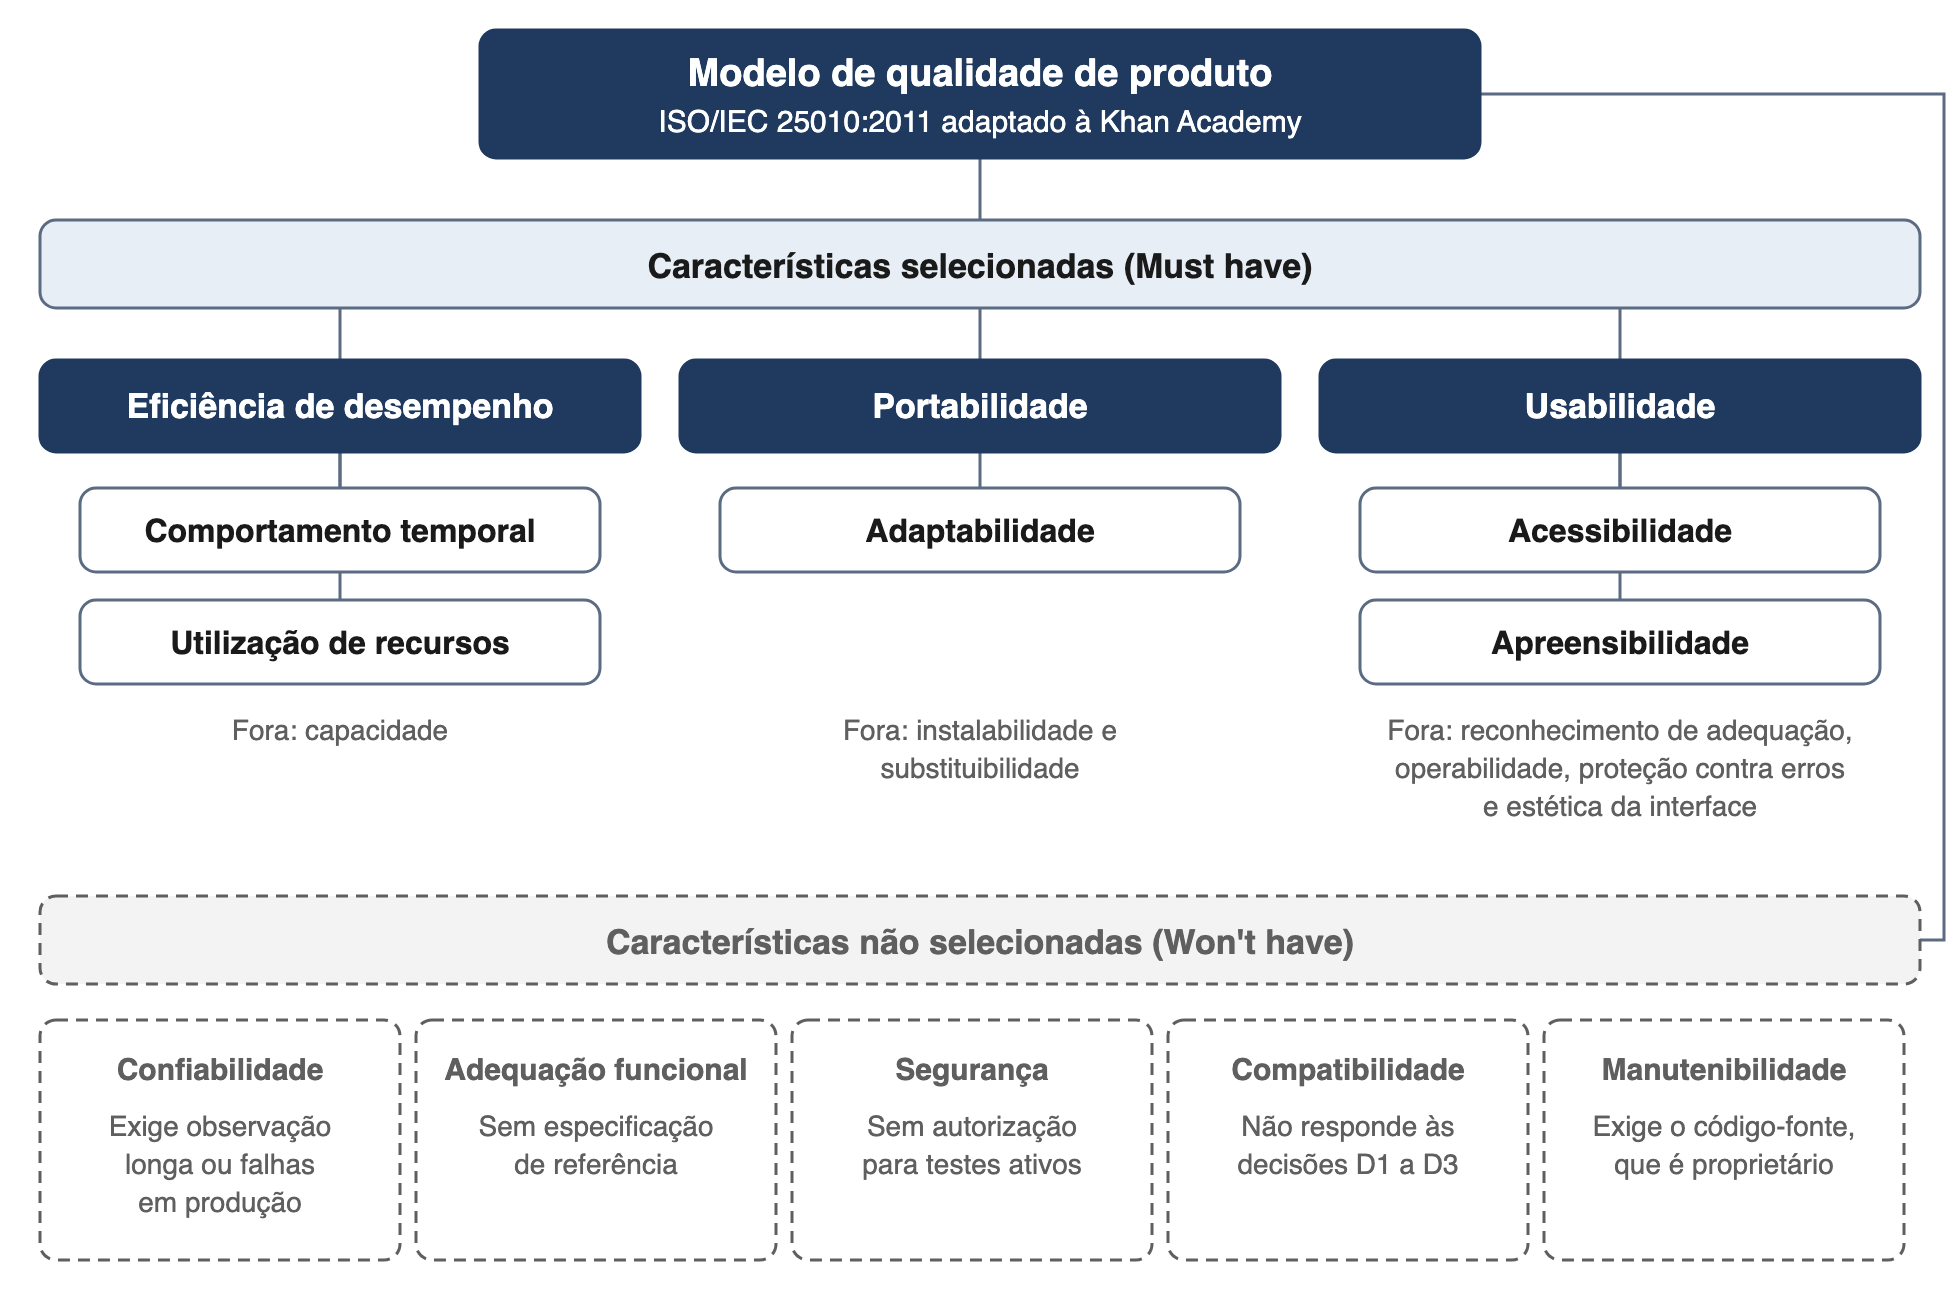
\includegraphics[width=0.6\textwidth]{figuras/modelo-qualidade.png}%
}{%
  \fbox{\parbox{0.9\textwidth}{\centering\small Inserir a figura do modelo de qualidade em figuras/modelo-qualidade.png}}%
}
\caption{Modelo de qualidade adaptado da ISO/IEC 25010:2011 para a avaliação da Khan Academy}
\label{fig:modelo}
\end{figure*}

\subsection{Seleção e Priorização das Características}

A seleção aplicou uma matriz ponderada às oito características da ISO/IEC 25010:2011. Cada característica recebeu notas de 1 a 3 em impacto no aluno, risco no contexto do cenário e viabilidade de produzir evidência externa, combinadas na pontuação $P = 3I + 2R + V$, com máximo de 18. O impacto recebeu o maior peso porque o propósito é apoiar decisões sobre os alunos, e a viabilidade o menor, para que a facilidade de medir não determine sozinha a seleção.

A pontuação foi convertida em classes MoSCoW: \textit{Must have} para $P \geq 15$, \textit{Should have} para $12 \leq P \leq 14$, \textit{Could have} para $10 \leq P \leq 11$ e \textit{Won't have} para $P \leq 9$. Uma característica com viabilidade 1 também é classificada como \textit{Won't have}, pois a equipe não consegue produzir evidência sobre ela. A Tabela~\ref{tab:moscow} apresenta o resultado.

\begin{table}[htbp]
\centering
\caption{Seleção das características por MoSCoW com pesos}
\label{tab:moscow}
\scriptsize
\setlength{\tabcolsep}{4pt}
\begin{tabular}{lccccl}
\hline
\textbf{Característica} & \textbf{I} & \textbf{R} & \textbf{V} & \textbf{P} & \textbf{Classe} \\
\hline
Eficiência de desempenho & 3 & 3 & 3 & 18 & \textit{Must have} \\
Portabilidade & 3 & 2 & 2 & 15 & \textit{Must have} \\
Usabilidade & 3 & 2 & 2 & 15 & \textit{Must have} \\
Confiabilidade & 2 & 2 & 1 & 11 & \textit{Won't have} \\
Adequação funcional & 2 & 1 & 1 & 9 & \textit{Won't have} \\
Segurança & 2 & 1 & 1 & 9 & \textit{Won't have} \\
Compatibilidade & 1 & 1 & 2 & 7 & \textit{Won't have} \\
Manutenibilidade & 1 & 1 & 1 & 6 & \textit{Won't have} \\
\hline
\end{tabular}
\par\smallskip
{\scriptsize I: impacto no aluno (peso 3); R: risco no contexto (peso 2); V: viabilidade de evidência (peso 1).}
\end{table}

A confiabilidade alcança 11 pontos, mas sua avaliação exigiria observação prolongada do serviço ou indução de falhas em produção, o que não é autorizado. Adequação funcional exigiria uma especificação de referência indisponível e se confunde com a avaliação do conteúdo pedagógico; segurança exigiria autorização para testes ativos; compatibilidade não responde às decisões D1 a D3; e manutenibilidade depende do código-fonte, que é proprietário.

Nas três características selecionadas, foram mantidas cinco subcaracterísticas. Ficaram de fora capacidade, que exigiria gerar carga no servidor; instalabilidade e substituibilidade, que não se aplicam a uma plataforma web; e reconhecimento de adequação, operabilidade, proteção contra erros do usuário e estética da interface, que não apoiam nenhuma decisão do cenário ou já estão parcialmente cobertas pela acessibilidade e pela apreensibilidade.

A mesma matriz definiu a prioridade das subcaracterísticas selecionadas: prioridade alta para $P \geq 15$ e média para $12 \leq P \leq 14$. Cada subcaracterística originou um requisito de avaliação, de R1 a R5, apresentado na Tabela~\ref{tab:priorizacao} com a decisão apoiada e o objetivo GQM que dele deriva na Fase 2. As subcaracterísticas de prioridade alta recebem mais ambientes e repetições de medição; a apreensibilidade, de prioridade média, é avaliada com uma amostra exploratória.

\begin{table}[htbp]
\centering
\caption{Priorização das subcaracterísticas e requisitos de avaliação}
\label{tab:priorizacao}
\scriptsize
\setlength{\tabcolsep}{2.5pt}
\begin{tabular}{llccccccc}
\hline
\textbf{ID} & \textbf{Subcaracterística} & \textbf{I} & \textbf{R} & \textbf{V} & \textbf{P} & \textbf{Prior.} & \textbf{Dec.} & \textbf{Obj.} \\
\hline
R1 & Comportamento temporal & 3 & 3 & 3 & 18 & Alta & D1 & G1 \\
R2 & Utilização de recursos & 3 & 3 & 2 & 17 & Alta & D1 & G1 \\
R3 & Adaptabilidade & 3 & 2 & 2 & 15 & Alta & D1 & G2 \\
R4 & Acessibilidade & 3 & 2 & 2 & 15 & Alta & D2 & G3 \\
R5 & Apreensibilidade & 2 & 2 & 2 & 12 & Média & D3 & G3 \\
\hline
\end{tabular}
\end{table}

Como os pesos e as notas são critério da equipe, as pontuações foram recalculadas em dois cenários alternativos: com pesos iguais ($I + R + V$) e sem o critério de viabilidade ($3I + 2R$). Nos dois cenários, as três características selecionadas permanecem à frente das demais e a ordem das subcaracterísticas não se altera, o que indica que a seleção e a priorização não dependem de um ajuste fino dos pesos.

\subsection{Escopo, Profundidade e Limites de Validade}

O objeto da avaliação é a plataforma web acessada por navegadores em computadores, observada como caixa-preta. Os ensaios usam quatro fluxos: navegação em cursos (FL1), reprodução de videoaulas (FL2) e resolução de exercícios (FL3), que formam a jornada central de estudo e recebem maior profundidade, e consulta ao progresso do estudante (FL4), considerado secundário. A autenticação é apenas precondição, realizada com uma conta de teste controlada pela equipe.

Em vez de combinar todos os sistemas e navegadores, foram definidos quatro ambientes com finalidade específica, que cobrem os três motores de renderização (Blink, Gecko e WebKit): A1, Windows com Chrome, ambiente de referência, com NVDA, teclado, zoom de 200\% e alto contraste; A2, Windows com Firefox, com teclado; A3, macOS com Safari, com VoiceOver e teclado; e A4, Ubuntu LTS com Firefox, com Orca e teclado. Windows e macOS são executados em computadores reais; o Ubuntu pode ser executado em computador real ou em máquina virtual, com a modalidade e os recursos registrados antes da coleta.
Comportamento temporal e utilização de recursos são medidos apenas no ambiente de referência A1, com uma execução de aquecimento e cinco repetições válidas por tarefa, em conexão sem limitação artificial e em um perfil controlado de conexão limitada. A adaptabilidade é verificada nos quatro ambientes, nas resoluções de 1366 por 768 e 1920 por 1080 pixels. A acessibilidade combina navegação por teclado e leitores de tela nos ambientes A1, A3 e A4, com inspeções de zoom e alto contraste em A1 e inspeção automatizada apenas como apoio. A apreensibilidade é observada com três a cinco participantes adultos sem experiência prévia com a plataforma.

Ficam fora do escopo os aplicativos nativos, os navegadores móveis, os painéis de professores, responsáveis e administradores, a infraestrutura interna e as APIs não documentadas, os testes ativos de segurança, os testes de carga e disponibilidade dos servidores e a qualidade pedagógica do conteúdo. Os resultados valem apenas para os fluxos, versões, computadores, condições de rede e tecnologias assistivas efetivamente avaliados; os ensaios de acessibilidade não comprovam conformidade integral com a WCAG \cite{wcag21}, e a amostra de apreensibilidade não representa estatisticamente os estudantes de escolas públicas.

\subsection{Relação com os Objetivos de Desenvolvimento Sustentável}

O estudo relaciona-se de forma contextual com o ODS 4, Metas 4.5 e 4.a, e com o ODS 10, Meta 10.2 \cite{un_sdg4_5,un_sdg4_a,un_sdg10_2}. A Meta 4.5 trata da eliminação de disparidades e do acesso à educação para grupos vulneráveis, incluindo pessoas com deficiência; os ensaios de acessibilidade e apreensibilidade podem identificar barreiras técnicas ao localizar conteúdos, assistir a aulas e resolver exercícios. A Meta 4.a trata de instalações de ensino inclusivas, e seu indicador 4.a.1 mede a proporção de escolas com computadores, internet e materiais adaptados para estudantes com deficiência, condição que o cenário pressupõe. A Meta 10.2 trata da inclusão social e econômica, e os ensaios de eficiência e adaptabilidade em computadores e conexões limitados podem revelar barreiras técnicas de acesso. Essa relação é contextual: a avaliação caracteriza a qualidade do software e não mede os indicadores oficiais de educação, renda ou inclusão.

\section{Fase 2 - Especificação da Avaliação}

\subsection{Objetivos GQM}

Os objetivos de medição foram definidos a partir dos requisitos de qualidade priorizados na Fase 1, contemplando eficiência de desempenho, portabilidade e usabilidade. A especificação seguiu a abordagem GQM, considerando cinco elementos: objeto de análise, propósito, foco de qualidade, ponto de vista e contexto. A partir dessa estrutura, foram estabelecidos três objetivos, associados às características e subcaracterísticas selecionadas.

\subsubsection{G1 - Eficiência de Desempenho}

O objetivo G1 visa avaliar o desempenho observável dos fluxos
de navegação em cursos (FL1), videoaulas (FL2) e exercícios (FL3) da
Khan Academy, considerando o comportamento temporal e a
utilização de recursos computacionais. A análise contempla
a perspectiva de estudantes, professores, coordenação
escolar e responsáveis, em ambientes web com configurações
de hardware e condições de rede documentadas. Esse objetivo
está associado aos requisitos R1 e R2, às questões Q1 a Q4
e às métricas M1 a M5.

\subsubsection{G2 - Portabilidade}
O objetivo G2 concentra-se na avaliação da adaptabilidade
da Khan Academy aos ambientes computacionais contemplados
pelo estudo. São considerados os fluxos FL1 a FL4, sob a perspectiva de estudantes, professores
e coordenação escolar. A investigação abrange a execução
dessas funcionalidades nas combinações viáveis de
navegadores e sistemas operacionais de computadores
definidas no escopo. O objetivo corresponde ao requisito
R3, às questões Q5 e Q6 e às métricas M6 e M7.

\subsubsection{G3 - Usabilidade}

O objetivo G3 busca avaliar as condições de utilização
da plataforma, com ênfase na acessibilidade e na
apreensibilidade dos fluxos de navegação em cursos, videoaulas
e exercícios (FL1 a FL3). A análise considera estudantes com
baixa visão ou que utilizam leitores de tela, estudantes
sem experiência prévia com a plataforma, professores
e responsáveis. O contexto de avaliação compreende a
versão web da Khan Academy, incluindo a utilização de
recursos de navegação por teclado e tecnologias assistivas
compatíveis com os ambientes selecionados, além de
procedimentos relacionados à aprendizagem da interface.
Esse objetivo está associado aos requisitos R4 e R5,
às questões Q7 a Q11 e às métricas M8 a M14.

A definição desses objetivos estabelece a rastreabilidade
entre os requisitos de qualidade e os elementos de medição,
fornecendo a base para a especificação das questões,
hipóteses e métricas da avaliação.

\subsection{Questões e Hipóteses}

Os três objetivos foram desdobrados em 11 questões (Q1 a Q11), cada
uma associada a uma hipótese de mesmo número (H1 a H11) e respondida
por ao menos uma métrica
(Tabelas~\ref{tab:qh-g1} a \ref{tab:qh-g3-complemento}).
As questões investigam se os fluxos permanecem utilizáveis nas
condições do cenário escolar, sem antecipar fórmulas de cálculo.
As hipóteses explicitam o resultado esperado, o ambiente em que será
verificado e o limite adotado. Todas são suposições de trabalho
formuladas antes da coleta e propostas para ratificação da equipe,
e não representam resultados observados.

Nas hipóteses, A1 a A4 designam os ambientes do estudo: Windows com
Chrome (A1), Windows com Firefox (A2), macOS com Safari (A3) e Ubuntu
com Firefox (A4). FL1 a FL4 designam os fluxos de navegação em cursos,
videoaulas, exercícios e consulta ao progresso pelo próprio estudante.
Eficiência de desempenho, ampliação, alto contraste e apreensibilidade
são avaliadas apenas em A1, ambiente de referência. Teclado e leitor
de tela são avaliados em A1, A3 e A4, e a adaptabilidade, nos quatro
ambientes.

\providecommand*{\tabrr}{\raggedright\let\\\tabularnewline}

\subsubsection{G1 -- Eficiência de Desempenho}

Q1 trata da espera percebida pelo estudante, enquanto Q2, Q3 e Q4
separam CPU, memória e dados de rede porque cada recurso pode limitar
o uso de forma independente em computadores e conexões restritos.
H1 a H4 restringem-se a A1, onde os recursos serão monitorados.
H1 considera duas condições de rede, uma sem limitação artificial
e outra com perfil controlado de conexão limitada, que representa
a preocupação do cenário escolar com a conectividade.

\begin{table}[htbp]
\centering
\caption{Questões e hipóteses de G1 -- Eficiência de Desempenho}
\label{tab:qh-g1}
\footnotesize
\setlength{\tabcolsep}{3pt}
\begin{tabular}{p{0.09\columnwidth}p{0.67\columnwidth}p{0.14\columnwidth}}
\hline
\textbf{Q} & \textbf{Questão e hipótese} & \textbf{Métricas} \\
\hline
\tabrr Q1 &
\tabrr \textit{A espera por carregamentos, início de videoaulas e respostas de exercícios permite continuar a atividade sem interrupções?}\par
H1: em A1, para cada etapa de FL1 a FL3 e condição de rede, a mediana do tempo de resposta será de até 3 s e pelo menos 90\% das tentativas elegíveis serão concluídas, sem bloqueio atribuível à plataforma. &
\tabrr M1, M2 \\
\hline
\tabrr Q2 &
\tabrr \textit{Os fluxos podem ser concluídos sem sobrecarregar o processamento do computador de referência?}\par
H2: em A1, a utilização média de CPU será de até 50\% em cada execução válida de FL1 a FL3, sem interrupção atribuível à sobrecarga. &
\tabrr M3 \\
\hline
\tabrr Q3 &
\tabrr \textit{Os fluxos permanecem utilizáveis dentro da memória disponível?}\par
H3: em A1, o pico de memória será de até 1.024 MiB em cada execução válida de FL1 a FL3, sem interrupção atribuível ao esgotamento de memória. &
\tabrr M4 \\
\hline
\tabrr Q4 &
\tabrr \textit{O volume de dados do trecho padronizado de navegação é compatível com o orçamento de acesso?}\par
H4: em A1, cada execução concluída do trecho padronizado, com política de cache constante, transferirá no máximo 10 MiB, somando envio e recebimento. &
\tabrr M5 \\
\hline
\end{tabular}
\end{table}

A verificação exige que o tempo pedagógico de assistir à videoaula
ou resolver o exercício seja excluído de M1, que falhas e interrupções
sejam registradas à parte e que M5 considere apenas execuções
concluídas, com a mesma política de cache e sem transferência integral
de vídeos. Como H3 trata de picos, médias ou medianas de memória não
podem ocultar violações individuais. A coincidência entre CPU elevada
e interrupção não demonstra relação de causa isoladamente, e a
classificação segue o protocolo de evidências.


\subsubsection{G2 -- Portabilidade}

Q5 verifica se os fluxos são concluídos entre sistemas operacionais
e navegadores, e Q6 se conteúdo e controles se preservam nas resoluções
de referência. Ambas usam o mesmo patamar de 90\% das combinações
selecionadas, mas são contadas separadamente, de modo que um mesmo
resultado não seja computado duas vezes.

\begin{table}[htbp]

\centering
\caption{Questões e hipóteses de G2 -- Portabilidade}
\label{tab:qh-g2}
\footnotesize
\setlength{\tabcolsep}{3pt}
\begin{tabular}{p{0.09\columnwidth}p{0.67\columnwidth}p{0.14\columnwidth}}
\hline
\textbf{Q} & \textbf{Questão e hipótese} & \textbf{Métricas} \\
\hline
\tabrr Q5 &
\tabrr \textit{Os fluxos essenciais são concluídos nas combinações de sistema operacional e navegador, sem ajustes extraordinários na plataforma?}\par
H5: pelo menos 90\% das combinações de ambiente (A1 a A4) e fluxo (FL1 a FL4) selecionadas permitirão concluir o roteiro e alcançar o resultado esperado, sem alterar a plataforma. &
\tabrr M6 \\
\hline
\tabrr Q6 &
\tabrr \textit{Conteúdo e controles necessários permanecem utilizáveis nas resoluções avaliadas?}\par
H6: em pelo menos 90\% das combinações essenciais de ambiente, resolução (1366$\times$768 e 1920$\times$1080) e fluxo, as tarefas serão concluídas com acesso a todas as informações e controles do roteiro. &
\tabrr M7 \\
\hline
\end{tabular}
\end{table}

O protocolo deve distinguir a preparação normal do ensaio de um
ajuste extraordinário na plataforma. Combinações inviáveis por
incompatibilidade conhecida entre ferramentas e sistemas são tratadas
no planejamento e não contam automaticamente como falha da
Khan Academy.

\FloatBarrier
\subsubsection{G3 -- Usabilidade}

Q7 a Q10 abordam a acessibilidade por teclado, leitor de tela,
ampliação e contraste, tendo como referência critérios aplicáveis
da WCAG 2.1 \cite{wcag21}. Em H7, a conclusão ocorre sem substituir
o teclado pelo mouse durante a tarefa. Em H8, o resultado depende
do anúncio das informações e da identificação dos controles, e não
apenas da presença de rótulos. Q9 difere de Q6: avalia a ampliação
do conteúdo (zoom de 200\%), e não a mudança do tamanho da janela.
H10 reúne dois ramos independentes, porque o alto contraste do
Windows não substitui a verificação das razões de contraste.

As questões e hipóteses de G3 estão distribuídas nas
Tabelas~\ref{tab:qh-g3} e \ref{tab:qh-g3-complemento}.

\begin{table}[htbp]
\centering
\caption{Questões e hipóteses de G3: teclado, leitor de tela e ampliação}
\label{tab:qh-g3}
\footnotesize
\setlength{\tabcolsep}{3pt}
\begin{tabular}{p{0.09\columnwidth}p{0.67\columnwidth}p{0.14\columnwidth}}
\hline
\textbf{Q} & \textbf{Questão e hipótese} & \textbf{Métricas} \\
\hline
\tabrr Q7 &
\tabrr \textit{Quem usa apenas teclado consegue identificar e acionar os controles necessários, sem bloqueios?}\par
H7: em pelo menos 90\% das combinações de tarefa e ambiente (A1, A3 e A4) para FL1 a FL3, a tarefa será concluída apenas por teclado, com foco visível e sem bloqueios de navegação. &
\tabrr M8 \\
\hline
\tabrr Q8 &
\tabrr \textit{Quem usa leitor de tela recebe as informações necessárias e consegue concluir os fluxos?}\par
H8: em pelo menos 90\% das combinações com NVDA (A1), VoiceOver (A3) e Orca (A4), o leitor anunciará as informações e identificará os controles definidos no \textit{checklist}, permitindo concluir a tarefa sem consulta visual. &
\tabrr M9 \\
\hline
\tabrr Q9 &
\tabrr \textit{A ampliação permite continuar lendo o conteúdo e operando os controles, sem perda de informação ou funcionalidade?}\par
H9: em A1, a 1366$\times$768, pelo menos 90\% das tarefas essenciais serão concluídas com zoom de 200\%, sem perda das informações ou dos controles necessários. &
\tabrr M10 \\
\hline
\end{tabular}
\end{table}

\begin{table}[htbp]
\centering
\caption{Questões e hipóteses de G3: contraste e apreensibilidade}
\label{tab:qh-g3-complemento}
\footnotesize
\setlength{\tabcolsep}{3pt}
\begin{tabular}{p{0.09\columnwidth}p{0.67\columnwidth}p{0.14\columnwidth}}
\hline
\textbf{Q} & \textbf{Questão e hipótese} & \textbf{Métricas} \\
\hline
\tabrr Q10 &
\tabrr \textit{A apresentação visual permite distinguir informações e controles, inclusive em alto contraste?}\par
H10: (a) todos os textos aplicáveis inspecionados atenderão ao contraste mínimo de 4,5:1 (texto comum) e 3:1 (texto grande), e (b) em A1, pelo menos 90\% das tarefas essenciais serão concluídas com o alto contraste do Windows ativado, sem desativá-lo. &
\tabrr M11 \\
\hline
\tabrr Q11 &
\tabrr \textit{Estudantes novos conseguem iniciar e concluir as tarefas essenciais após a instrução inicial, sem orientação adicional?}\par
H11: em A1, pelo menos 90\% das primeiras tentativas elegíveis de cada tarefa essencial, e do conjunto avaliado, serão concluídas por participantes adultos novos na plataforma, após instrução inicial padronizada e sem ajuda. &
\tabrr M12, M13, M14 \\
\hline
\end{tabular}
\end{table}

Q11 aborda a apreensibilidade em caráter exploratório, com três a
cinco participantes adultos sem experiência anterior com a plataforma.
H11 considera apenas a primeira tentativa de cada par
participante--tarefa, após instrução inicial padronizada.
M12 é a métrica principal de Q11, e M13 (erros) e M14 (tempo) a
complementam, pois uma tarefa concluída autonomamente pode ainda
indicar dificuldade de aprendizagem. Se o recrutamento não for
possível, o resultado será apresentado como inspeção exploratória
da equipe, e não como evidência sobre estudantes.

\FloatBarrier
\subsubsection{Fundamentação e Verificação das Hipóteses}

As hipóteses derivam dos requisitos R1 a R5 e das restrições do
escopo. Os limites quantitativos, como 3 s em H1, 50\% em H2,
1.024 MiB em H3, 10 MiB em H4 e 90\% nas demais, são critérios
operacionais propostos pelo estudo, e não valores normativos da
ISO/IEC 25023 \cite{iso25023_2016}. Eles devem ser ratificados pela
equipe antes da coleta. A interpretação de cada hipótese confronta
os dados válidos com o seu enunciado, e não apenas com a pontuação
da métrica, e resulta em um de três estados:

\begin{itemize}
\item \textbf{Sustentada na amostra:} os dados válidos, com cobertura
suficiente, atendem integralmente à expectativa.
\item \textbf{Não sustentada na amostra:} os dados válidos e
suficientes não atendem à expectativa, e a divergência é
acompanhada da evidência.
\item \textbf{Inconclusiva:} faltam parâmetros fundamentados,
dados válidos ou cobertura necessária. Achados parciais permanecem
registrados.
\end{itemize}

Os resultados valem apenas para os fluxos, ambientes e condições
efetivamente avaliados e serão obtidos na etapa de coleta.
 
\subsection{Métricas de Avaliação}

As métricas foram definidas com base na abordagem
\textit{Goal-Question-Metric} (GQM), considerando as
características de qualidade selecionadas para a avaliação
da plataforma Khan Academy, em sua versão web, e a
ISO/IEC 25023:2016 \cite{iso25023} como referência para a especificação
das medidas.

Foram estabelecidas 14 métricas (M1 a M14), distribuídas
entre três objetivos: eficiência de desempenho (G1),
portabilidade (G2) e usabilidade (G3). A
Tabela~\ref{tab:metricas} apresenta os indicadores
propostos e sua associação às questões GQM, e a
Figura~\ref{fig:gqm} apresenta a hierarquia entre objetivos,
questões e métricas.

\begin{figure*}[t]
\centering
\IfFileExists{figuras/diagrama-gqm.png}{%
  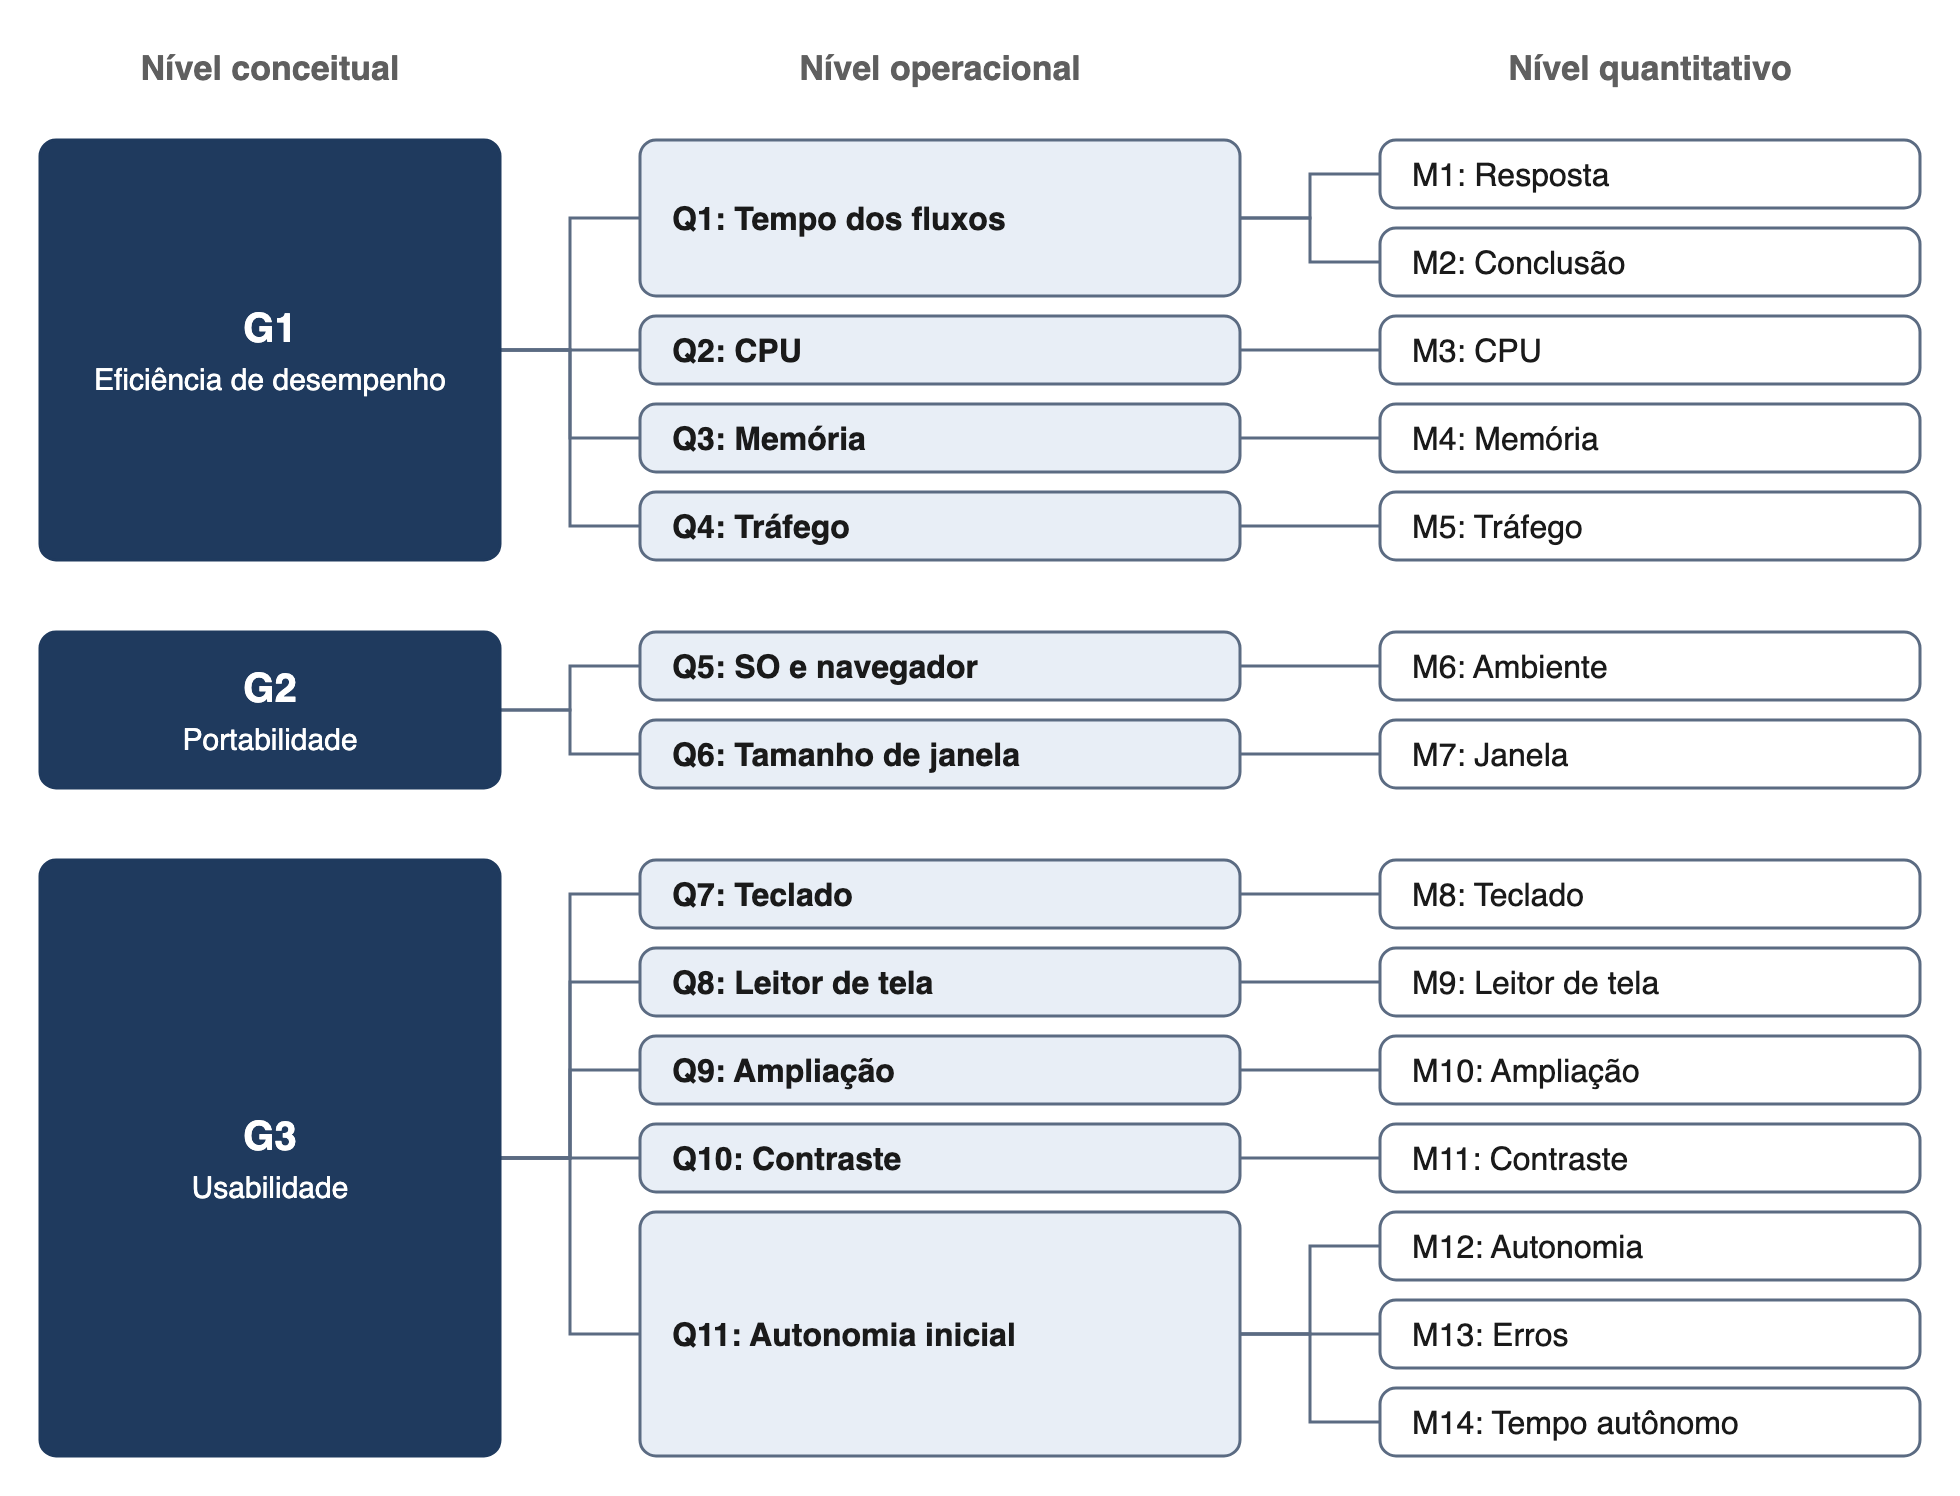
\includegraphics[width=0.6\textwidth]{figuras/diagrama-gqm.png}%
}{%
  \fbox{\parbox{0.9\textwidth}{\centering\small Inserir o diagrama GQM em figuras/diagrama-gqm.png}}%
}
\caption{Hierarquia GQM: objetivos G1 a G3, questões Q1 a Q11 e métricas M1 a M14}
\label{fig:gqm}
\end{figure*}


\begin{table}[htbp]
\centering
\caption{Métricas de avaliação da Khan Academy}
\label{tab:metricas}
\scriptsize
\setlength{\tabcolsep}{3pt}
\begin{tabular}{cllc}
\hline
\textbf{Obj.} & \textbf{Métrica} &
\textbf{Indicador} & \textbf{Q.} \\
\hline
G1 & M1: Resposta & Mediana/P90 (s) & Q1 \\
G1 & M2: Conclusão & Sucesso (\%) & Q1 \\
G1 & M3: CPU & Média (\%) & Q2 \\
G1 & M4: Memória & Pico (MiB) & Q3 \\
G1 & M5: Tráfego & Volume (MiB) & Q4 \\
G2 & M6: Ambiente & Sucesso (\%) & Q5 \\
G2 & M7: Janela & Adequação (\%) & Q6 \\
G3 & M8: Teclado & Conclusão (\%) & Q7 \\
G3 & M9: Leitor de tela & Conclusão (\%) & Q8 \\
G3 & M10: Ampliação & Adequação (\%) & Q9 \\
G3 & M11: Contraste & Conformidade (\%) & Q10 \\
G3 & M12: Autonomia & Conclusão (\%) & Q11 \\
G3 & M13: Erros & Taxa (\%) & Q11 \\
G3 & M14: Tempo autônomo & Mediana (s) & Q11 \\
\hline
\end{tabular}
\end{table}


A coleta será realizada em ambientes e fluxos previamente
definidos, utilizando registros de execução, instrumentos
de monitoramento e verificações de acessibilidade.
Os resultados quantitativos serão complementados pelo
registro de falhas e barreiras que comprometam
funcionalidades essenciais.

\FloatBarrier
\subsection{Critérios de Julgamento}

Para interpretar as medições, adotou-se uma escala
ordinal de quatro níveis: Excelente (3), Alvo (2),
Mínimo aceitável (1) e Inaceitável (0). Resultados
sem evidências suficientes serão classificados como
inconclusivos.

As métricas percentuais de sucesso incluem M2
(conclusão de fluxos), M6 (execução por ambiente),
M7 (adaptação ao tamanho da janela), M8 (navegação
por teclado), M9 (uso de leitor de tela), M10
(ampliação de conteúdo) e M12 (conclusão autônoma).
Os níveis correspondentes são apresentados na
Tabela~\ref{tab:criterios-percentuais}.

\begin{table}[htbp]
\centering
\caption{Critérios para métricas percentuais}
\label{tab:criterios-percentuais}
\small
\begin{tabular}{lcc}
\hline
\textbf{Nível} &
\textbf{M2, M6 a M10, M12} &
\textbf{M13} \\
\hline
Excelente (3) & $100\%$ & $0\%$ \\
Alvo (2) & $[90,100)\%$ & $(0,10]\%$ \\
Mínimo (1) & $[75,90)\%$ & $(10,25]\%$ \\
Inaceitável (0) & $<75\%$ & $>25\%$ \\
\hline
\end{tabular}
\end{table}

Para as métricas temporais e de utilização de recursos,
valores menores representam resultados mais favoráveis.
A Tabela~\ref{tab:criterios-recursos} apresenta os
limites operacionais estabelecidos.


\begin{table}[t]
\centering
\caption{Critérios para tempo e recursos}
\label{tab:criterios-recursos}
\scriptsize
\setlength{\tabcolsep}{3pt}
\begin{tabular}{lcccc}
\hline
\textbf{Métrica} & \textbf{3} & \textbf{2} &
\textbf{1} & \textbf{0} \\
\hline
M1 (s) & $\leq1$ & $(1,3]$ & $(3,10]$ & $>10$ \\
M3 (\%) & $\leq25$ & $(25,50]$ &
$(50,75]$ & $>75$ \\
M4 (MiB) & $\leq512$ & $(512,1024]$ &
$(1024,2048]$ & $>2048$ \\
M5 (MiB) & $\leq5$ & $(5,10]$ &
$(10,20]$ & $>20$ \\
M14 (s) & $\leq60$ & $(60,120]$ &
$(120,180]$ & $>180$ \\
\hline
\end{tabular}
\end{table}


A avaliação de acessibilidade considera requisitos
aplicáveis da WCAG 2.1 \cite{wcag21}. Para M10, será verificada a
preservação do conteúdo e das funcionalidades durante
a ampliação, incluindo o redimensionamento de texto
até 200\%. Para M11, serão considerados os limites
de contraste do nível AA (4,5:1 para textos comuns
e 3:1 para textos grandes) e do nível AAA
(7:1 e 4,5:1, respectivamente). Em M11, o
atendimento aos limites AA corresponde ao nível
Alvo (2), enquanto o atendimento aos limites AAA
corresponde ao nível Excelente (3). Falhas restritas
a elementos não essenciais ou que comprometam
elementos essenciais recebem, respectivamente,
pontuações 1 e 0.

As métricas M8 e M9 também consideram as barreiras
identificadas na navegação por teclado e na utilização
de leitores de tela, sem que os percentuais obtidos
impliquem conformidade integral com a WCAG.

Os limites quantitativos constituem critérios
operacionais propostos para o estudo, não valores
normativos da ISO/IEC 25023. A aplicação pressupõe
a padronização dos ambientes e fluxos, sendo M5
restrita à navegação sem transferência integral
de vídeos e M14 a tarefas curtas não pedagógicas.

Uma questão GQM será considerada atendida quando
suas métricas principais alcançarem pontuação igual
ou superior a 2, desde que não existam bloqueios
em funcionalidades essenciais. O atendimento de
cada objetivo dependerá do resultado de suas
questões, enquanto as hipóteses serão examinadas
com base nas evidências coletadas.

\section{Conclusão}

Este trabalho apresentou as duas primeiras fases da avaliação de qualidade da plataforma web da Khan Academy, conduzida segundo o processo de avaliação da família SQuaRE \cite{iso25040}. Na Fase 1, o propósito foi associado a um cenário de aplicação e a quatro decisões com responsáveis definidos; as características foram selecionadas por uma matriz ponderada convertida em classes MoSCoW, resultando em eficiência de desempenho, portabilidade e usabilidade; e o escopo foi delimitado a quatro fluxos e quatro ambientes, com limites de validade explícitos e relação contextual com os ODS 4 e 10. Na Fase 2, os cinco requisitos de avaliação foram desdobrados, pela abordagem GQM \cite{basili1994goal}, em três objetivos, 11 questões e 14 métricas, com critérios de julgamento em uma escala comum.

A principal contribuição desta etapa é a rastreabilidade entre o propósito, as decisões, os requisitos, os objetivos de medição e os critérios de julgamento, que permite interpretar os resultados futuros em relação às decisões que eles devem apoiar. O teste de sensibilidade mostrou que a seleção e a priorização não dependem do ajuste fino dos pesos definidos pela equipe.

O estudo tem limitações que orientarão a interpretação dos resultados: a avaliação é externa e de caixa-preta, o desempenho será medido em um único computador de referência, a amostra de apreensibilidade é exploratória e os limiares quantitativos são propostas metodológicas da equipe, e não valores normativos. Como próximos passos, as Fases 3 e 4 detalharão o plano de execução dos ensaios, realizarão a coleta das medidas nos ambientes definidos e analisarão os resultados à luz das hipóteses e dos critérios de julgamento, resultando em recomendações para a adoção da plataforma no cenário considerado.



\printbibliography

%%
%% If your work has an appendix, this is the place to put it.
\appendix

\section{Contribuição dos Integrantes}

A Tabela~\ref{tab:commands} apresenta a contribuição de cada integrante nas atividades da Entrega 1.

\begin{table*}[htbp]
  \centering
  \caption{Contribuição dos integrantes na Entrega 1}
  \label{tab:commands}
  \begin{tabular}{c l p{8cm} c}
    \toprule
    Matrícula & Integrante & Participação & Porcentagem de Contribuição \\
    \midrule
    \texttt{232013944} & Camila Silva Cavalcante & Questões e hipóteses; Níveis de pontuação e critérios de julgamento; Hierarquia e representação gráfica GQM & 16,6\% \\
    \texttt{241011054} & Enzo Menali Vettorato Toledo & Caracterização do produto; Contexto de uso; Stakeholders e perfis de estudantes & 16,6\% \\
    \texttt{232014450} & Geovanna Alves Umbelino & Objetivos de medição; Especificação das métricas; Níveis de pontuação e critérios de julgamento; Hierarquia e representação gráfica GQM & 16,7\% \\
    \texttt{231026429} & José Augusto Alves de Moraes & Escopo e objetos da avaliação; Ambientes de teste; Alinhamento com as ODS & 16,6\% \\
    \texttt{232014807} & Luísa de Souza Ferreira & Propósito, uso pretendido, modelo de qualidade e priorização das características, Referencial Teórico e Metodologia & 16,8\% \\
    \texttt{241025710} & Pedro Lucas Barbosa da Silva & Gestão PSM/CID; Organização e planejamento das issues; Estruturação do artigo; Revisão e Padronização do Pages & 16,7\% \\
    \midrule
    & & Total & 100\% \\
    \bottomrule
  \end{tabular}
\end{table*}


\end{document}
\endinput
%%
%% End of file `sigconf.tex'.
